\documentclass[12pt,a4paper]{article}

\usepackage[T1]{fontenc}
\usepackage[utf8]{inputenc}
\usepackage{polski}
\usepackage{lipsum}
\usepackage{amsmath}
\usepackage{graphicx}

\title{Ćwiczenie 3 - LaTeX podstawy pracy z procesorem tekstów (Zadanie 1)}
\author{Michał Gajda}
\date{22 October 2025}

\begin{document}

\maketitle

\newpage
\section{Formatowanie tekstu}

\begin{center}
\lipsum[1]
\end{center}

\begin{center}
\lipsum[2]
\end{center}

\begin{center}
\lipsum[3]
\end{center}

\begin{center}
\lipsum[4]
\end{center}

\begin{flushright}
\lipsum[5]
\end{flushright}

\begin{flushright}
\lipsum[6]
\end{flushright}

\begin{flushright}
\lipsum[7]
\end{flushright}

\begin{flushleft}
\lipsum[8]
\end{flushleft}

\begin{flushleft}
\lipsum[9]
\end{flushleft}

\begin{flushleft}
\lipsum[10]
\end{flushleft}

{\tiny Michał Gajda 346948}

{\small Michał Gajda 346948}

{\normalsize Michał Gajda 346948}

{\large Michał Gajda 346948}

{\huge Michał Gajda 346948}

{\rmfamily Michał Gajda 346948} % Tekst w kroju szeryfowym lub \textrm{...}

{\bfseries Michał Gajda 346948} % Tekst w kroju pogrubionym lub \textbf{...}

{\itshape Michał Gajda 346948} % Tekst kursywą lub \textit{...}

{\scshape Michał Gajda 346948} % Tekst kapitalikowy lub \textsc{...}

% \begin{scshape}
% ...
% \end{scshape}

\newpage
\section{Listy}

\begin{itemize}
\item Phaal
\item Vindaloo
\item Tikka Masala
\item Zupa ogórkowa
\end{itemize}

\begin{enumerate}
\item Die Hard
\item Die Hard 2: Die Harder
\item Die Hard with a Vengeance
\end{enumerate}

\newpage
\section{Wzory}

\begin{equation} % a) w trybie eksponowanym z numeracją (ze zdefiniowaną etykietą)
\label{eq:wzor1}
\hat{\sigma}^2_f = \frac{1}{(N - 1)} \left[\frac{1}{N} \sum_{i=1}^{N} f^2(x_i) - \left(\frac{1}{N} \sum_{i=1}^{N} f(x_i)\right)^2\right]
\end{equation}

\[ % b) w trybie eksponowanym
\hat{\sigma}^2_f = \frac{1}{(N - 1)} \left[\frac{1}{N} \sum_{i=1}^{N} f^2(x_i) - \left(\frac{1}{N} \sum_{i=1}^{N} f(x_i)\right)^2\right]
\]

$\hat{\sigma}^2_f = \frac{1}{(N - 1)} \left[\frac{1}{N} \sum_{i=1}^{N} f^2(x_i) - \left(\frac{1}{N} \sum_{i=1}^{N} f(x_i)\right)^2\right]$ % c) w trybie wierszowym

W LaTeX mamy trzy różne sposoby wstawiania wzorów, pierwsze podejście pozwala na odwoływanie się do wzoru po jego identyfikatorze (np: \eqref{eq:wzor1}), drugie podejście prezentuje wzór osobnej linii a trzecie pozwala na umieszczenie takiego wzoru w treści tekstu (np: $f(x) = x^2$).

\newpage
\section{Tabela}

\begin{table}[h]
\centering
\caption{Przykładowa tabela}
\label{tab:tab1}
\begin{tabular}{|c|l|r|}
\hline
Kolumna 1 & Kolumna 2 & Kolumna 3 \\
\hline
1 & 1 & 1 \\
2 & 2 & 2 \\
3 & 4 & 5 \\
\hline
\end{tabular}
\end{table}

\newpage
\section{Rysunki}

\begin{figure}[h]
\centerline{
	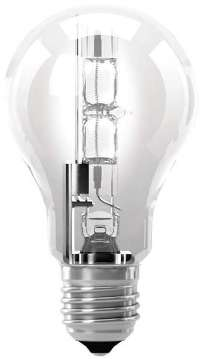
\includegraphics{Rysunek2.jpg}
}
\caption{Żarówka}
\label{rys1}
\end{figure} 

\begin{figure}
\centerline{
	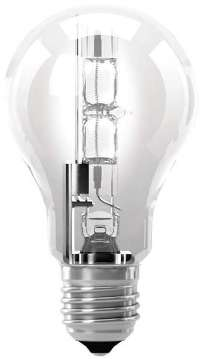
\includegraphics[scale=0.35]{Rysunek2.jpg}
}
\caption{Żarówka}
\label{rys2}
\end{figure}

\begin{figure}
\centerline{
	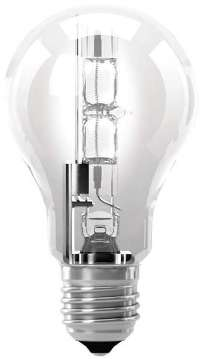
\includegraphics[angle=30]{Rysunek2.jpg}
}
\caption{Żarówka}
\label{rys3}
\end{figure}

\clearpage
\section{Podsumowanie}

Nauczyłem się, jak za pomocą LaTeX-a tworzyć dokumenty zawierające różnego typu obiekty, do których mogę się odwoływać — na przykład do wzoru \ref{eq:wzor1}, tabeli \ref{tab:tab1} oraz obrazka \ref{rys1}.
Łatwość, z jaką korzysta się z LaTeX-a, wręcz onieśmiela — w porównaniu z tym praca w Microsoft Wordzie to czysty masochizm.
Dodatkowo możliwe jest przechowywanie kodu takiego dokumentu w repozytorium Git i automatyczne generowanie plików za pomocą GitHub Actions.

\end{document}
